\documentclass[t]{beamer}

\usepackage[slovene]{babel}
\usepackage[T1]{fontenc}
\usepackage[utf8]{inputenc}
\usepackage{amssymb}
\usepackage{amsmath}


\usepackage{lmodern}                           
\renewcommand\textbullet{\ensuremath{\bullet}}
\title{Krožnica v racionalni Bezierjevi obliki}
\author{Anja Kišek, Samo Kralj}

\usetheme{CambridgeUS}

\begin{document}
%%%%%%%%%%%%%%%%%%%%%%%%%%%%%%%%%%%%%%
\begin{frame}
\titlepage
\end{frame}

%%%%%%%%%%%%%%%%%%%%%%%%%%%%%%%%%%%%%

\begin{frame}
Vsebina:
\begin{itemize}
\item Definicija racionalnih Bezierjevih krivulj

\item Konstrukcija sklenjene krožnice s krivuljami stopnje 2,3,4

\item Krožni loki v racionalni Bezierjevi obliki

\item Kubični polkrogi

\end{itemize}

\end{frame}
%%%%%%%%%%%%%%%%%%%%%%%%%%%%%%%%%%%%
\begin{frame}
Racionalna Bezierjeva krivulja $C(t)$ stopnje $n$ v $\mathbb{R}^d$ je projekcija polinomske Bezierjeve krivulje $\tilde{C}(t)$stopnje $n$ v $\mathbb{R}^{d+1}$ na hiperravnino $w=1$, kjer je točka v $\mathbb{R}^{d+1}$ označena z $
\begin{bmatrix} x \\ w \end{bmatrix}.$


Racionalna B. krivulja stopnje $n$ je tako podana s predpisom
$$r(t) = \frac{\sum_{i=0}^n w_ib_iB_i^n(t)}{\sum_{i=0}^n w_iB_i^n(t)} $$

\end{frame}
%%%%%%%%%%%%%%%%%%%%%%%%%%%%%
\begin{frame}
Racionalna krivulja $C(t) = (X(t), Y(t))$ lahko eksaktno opiše krožnico kot projekcijo krivulje
$\tilde{C}(t) = (\tilde{X}(t), \tilde{Y}(t), W(t)),$ ki leži na stožcu, na ravnino $w = 1$.

\begin{align*}
X(t)^2 + Y(t)^2 &= 1 \\
\Big{(}\frac{\tilde{X}(t)}{W(t)}\Big{)}^2 + \Big{(}\frac{\tilde{Y}(t)}{W(t)}\Big{)}^2 &= 1\\
\tilde{X}(t)^2 + \tilde{Y}(t)^2 - W(t)^2 &= 0
\end{align*}
\begin{figure}
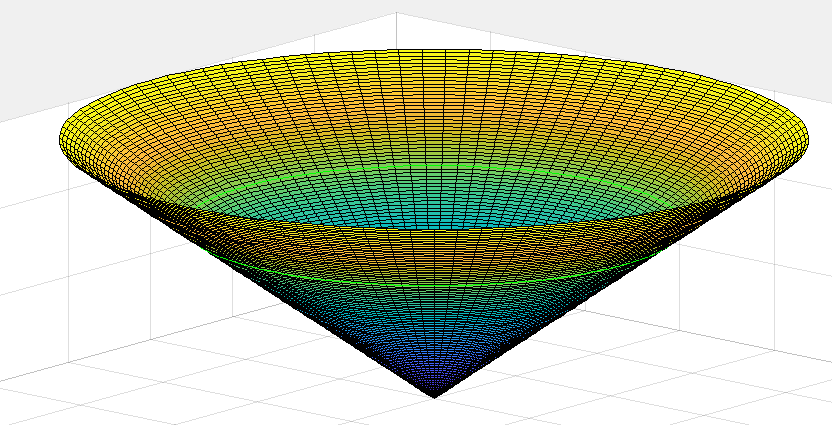
\includegraphics[scale=0.2]{stozec.png}
\end{figure}

\end{frame}

%%%%%%%%%%%%%%%%%%%%%%%%%%%%%

\begin{frame}
\textbf{Bezierjeva krivulja kot sklenjena krožnica}

Ali lahko krožnico zapišemo kot racionalno Bezierjevo krivuljo določene stopnje?
\begin{itemize}
\item Kvadratična krivulja: Ne

Zlepek krožnih lokov s kontrolnimi točkami:
\begin{align*}
\tilde{P}_0 &= (cos(\phi), -sin(\phi), 1)\\
\tilde{P}_1 &= (1, 0, cos(\phi))\\
\tilde{P}_2 &= (cos(\phi), sin(\phi), 1)
\end{align*}

\item Kubična krivulja: Ne
\end{itemize}
\end{frame}
%%%%%%%%%%%%%%%%%%%%%%%%%%%%%%%%%%%%%%
\begin{frame}
\begin{itemize}
\item Krivulja 4. stopnje: reševanje sistema 9 enačb
\begin{align*}
\tilde{y}_3 + \tilde{y}_1 &= 0\\
\tilde{x}_3 + \tilde{x}_1 &= 0\\
3\tilde{x}_2 + 4\tilde{y}_1^2 - 3w_3 &= 0 \\
\tilde{x}_1\tilde{x}_2 + \tilde{y}_1\tilde{y}_2  - \tilde{x}_1w_2 &= 0 \\
9\tilde{x}_2^2 - 8\tilde{y}_1^2 + \tilde{y}_2^2 - 9w_2^2&= 0 \\
\end{align*}
Za $\alpha = (\frac{3w_2}{2} - \tilde{x}_1^2 + \frac{1}{2})^{\frac{1}{2}}$ dobimo dva kontrolna poligona
\begin{align*}
\tilde{P}_0 &= (1,0, 1)\\
\tilde{P}_1 &= (\tilde{x}_1, \pm \alpha,\tilde{x}_1)\\
\tilde{P}_2 &= (-\frac{3w_2 - 4\tilde{w}_1^2+2}{3}, \pm \frac{3}{4}\tilde{x}_1\alpha, w_2)\\
\tilde{P}_3 &= (-\tilde{x}_1, \mp \alpha,-\tilde{x}_1)\\
\tilde{P}_4 &= (1,0,1) \\
\end{align*}
\end{itemize}

\end{frame}
%%%%%%%%%%%%%%%%%%%%%%%%%%%%%%%%%
\begin{frame}
\begin{itemize}
\item Krivulja 4. stopnje: uteži so lahko negativne ali ničelne
\item Krivulja 5. stopnje: s pomočjo višanja stopnje

Primer:
\begin{columns}
	\column{0.5\linewidth}
	\begin{align*}
	\tilde{P}_0 &= (1,0, 1)\\
	\tilde{P}_1 &= (0, 1, 0)\\
	\tilde{P}_2 &= (-1, 0, 1/3)\\
	\tilde{P}_3 &= (0, -1, 0)\\
	\tilde{P}_4 &= (1, 0, 1) \\
	\end{align*}
	\column{0.5\linewidth}
    \begin{align*}
	\tilde{P}_0 &= (1,0, 1)\\
	\tilde{P}_1 &= (1/5, 4/5, 1/5)\\
	\tilde{P}_2 &= (-3/5, 2/5, 1/5)\\
	\tilde{P}_3 &= (-3/5, -2/5, 1/5)\\
	\tilde{P}_4 &= (1/5, -4/5, 1/5)\\
	\tilde{P}_5 &= (1, 0, 1) \\
	\end{align*}
\end{columns}

\end{itemize}
\end{frame}


\end{document}
